\chapter{Related Work}

This section is the result of researching existing academic and commercial software systems and publications.
Since no prior systems with these requirements could be determined, related work was sought to cover subproblems
related to the design and implementation of such a system.

The section starts by the revision of three academic solutions with common goals with the proposed solution:
Arvika, Multi-User Tabletop Speech and Gestures and Digital Whiteboard.
An analysis is then conducted regarding input and output modalities capable of enabling such scenarios,
along with a set of shape creation and scene navigation techniques.
A comparative analysis of commercially available building modeling software is then conducted.
The section ends with the result of two interviews gathered with architects in order to survey
building characteristics and possible improvements over the common architectural work flow.


\section{Existing Solutions}

% EXISTING SOLUTIONS
% existing solutions

% intro

Three systems will be discussed in this area, each one 
withstanding common goals with the idealized solution.

ARVIKA is the biggest project so far in the
Augmented Reality domain. It offers a working solution to aid in industrial tasks but leaves most
of the regular user interfaces intact, leaving space for improvements at this level.
Additionally, it lacks an authoring tool to provide end-users means to set up scenarios in a friendlier manner.

Speech and Gestures shows a project where the Google Earth \cite{SITE-EARTH} application
-- a single user system that allows navigation in a world representation -- has been adapted to
work on a multi-touch surface with speech recognition.
The adapting work provided feedback about the limitations such software faces 
and offers a working solution to map most Google Earth actions to speech and gesture commands.

Finally, Digital Whiteboard provides a solution for multi-user digital
whiteboards where each user handles a palmtop serving as both the user's palette and
private composing area, supporting text and drawings input.
A technique called pick-and-drop is then explained. It is used to allow a user to transfer
the contents of the palmtop on the shared whiteboard.

\TODOL{SEE NEWEST ARTICLE REPOSITORY, NAMELY instant architecture and IPCity}


\subsection{ARVIKA, 2003}

ARVIKA \cite{ARVIKA} is a project with sponsoring from the
German Federal Ministry of Education and Research that was implemented between 1999 and 2003.
It focused on the development of Augmented Reality (AR) technologies to aid in performing industrial tasks.
The consortium involved several industrial partners such as Volkswagen, BMW, Siemens and Airbus.

\begin{figure}[!ht]
    \centering
    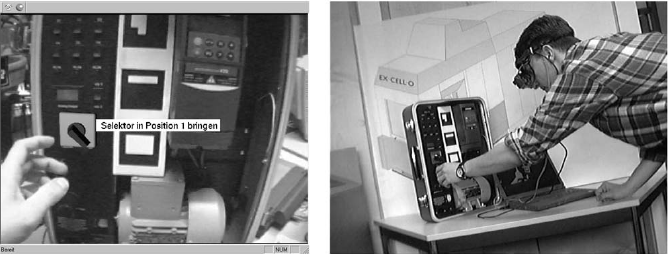
\includegraphics[width=10cm]{gfx/arvika.png}
    \caption{The augmented view seen from the HMD; a user of the ARVIKA system}
    \label{FIG-ARVIKA}
\end{figure}

An expert in the industrial area would carry a head-mounted display (HMD) with a camera mounted on it.
The real-time captured video was then interpreted and markers extracted from the image.
The camera's positioning and orientation were estimated and the HMD view was enriched with virtual objects
(see figure \ref{FIG-ARVIKA}, left).
The framework was distributed in the form of an ActiveX plug-in for the Internet Explorer browser
named ARBrowser.

% discussion

Weidenhausen et al. \cite{ARVIKA-LESSONS} consider the deployment of the project as an ActiveX component
to be an advantage since it is based on a widespread program (Internet Explorer) and allowed developers
to create task scenarios with familiar technologies such as JavaScript and HTML.
Although the world's largest research project in the area, ARVIKA focused too much on the technical problems
regarding AR and little effort was spent on the creation of a suitable user interface.
The authors agree on a point: ``most people judge the usefulness of a technology mainly by its user interface''.
Therefore this particular topic became work for future project iterations.
ARVIKA was meant to support many industrial scenarios -- development, production and services for several
industrial partners on different domains.
Creating a scenario was a time consuming task -- taking several days, according to Weidenhausen et al.
-- and required extensive knowledge in 3D modeling tools and VRML. No authoring capabilities were given to end-users.
This problem was identified as paramount and an authoring tool was scheduled for future development,
supporting generic task creation with parameters controlled by the users.



\subsection{Speech and Gestures on a Multi-User Tabletop, 2006}

Tse et al. \cite{SP-GEST-TTOP} developed a multimodal interface on top of Google Earth \cite{SITE-EARTH}
to be run on a multi-touch table.
The system allows multi-user collaboration with touch and voice commands.

The main problems found in adapting Google Earth reside in the fact that it was thought out as a single user program,
where only one action could be done at a time.
In this scenario several users could be disposed around the table with different orientations,
so text readability problems arose.
Additionally, user interface components such as the compass were placed at fixed points on the screen,
an approach that does not favor multi-user scenarios.
At 1024 x 768 resolution it was estimated that 42\% of the screen was originally consumed by GUI elements.
Since all users shared the surface, turn-taking had to be agreed by the users,
not being enforced by the system (see figure \ref{FIG-SP-TABLETOP}).
Most Google Earth interactive actions were mapped into gestures,
leaving the most abstract actions for voice commands activation (see figure \ref{FIG-SP-TABLETOP2}).


\begin{figure}[!ht]
    \centering
    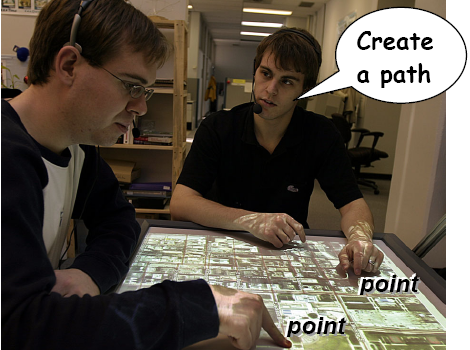
\includegraphics[width=7cm]{gfx/sp-gest-ttop.png}
    \caption{Two users collaborating on a Google Earth tabletop session}
    \label{FIG-SP-TABLETOP}
\end{figure}

\begin{figure}[!ht]
    \centering
    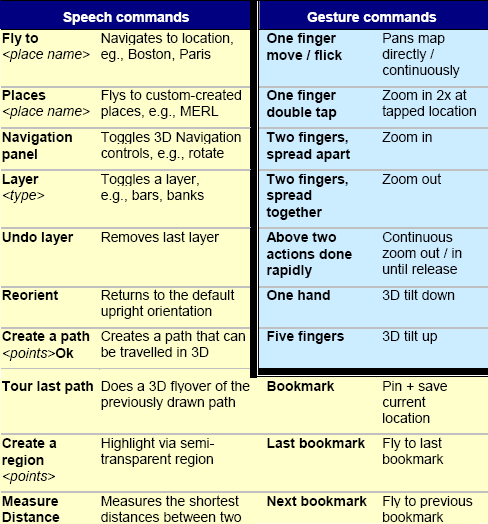
\includegraphics[width=8cm]{gfx/sp-gest-ttop2.png}
    \caption{The suggested speech and gesture interface for Google Earth}
    \label{FIG-SP-TABLETOP2}
\end{figure}

%\paragraph{Discussion}

This project shows the difficulties in adapting a production software thought out
for single user WIMP\footnote{Window Icon Menu Pointing device} interfaces for the support of collaborative scenarios.
A multimodal interface was built over the existing one, mapping most of its commands.
The set of obtained commands is a good example of how navigation can be performed on
3D scenery using a multimodal interface.
Google Earth is a good example of a navigation system suited for single user interaction.
It provides several functionality and could support the creation of buildings.
Making use of its large dataset of satellite images and topography would be excellent
for the target system.


\subsection{Digital Whiteboard, 1998}

Rekimoto \cite{WBOARD} presents a digital whiteboard where each participant is given
a palmtop computer to handle. It works as a tool palette, remote commander, text entry box as
well as a temporary data buffer during whiteboard collaboration interaction.

\begin{figure}[!ht]
	\centering
	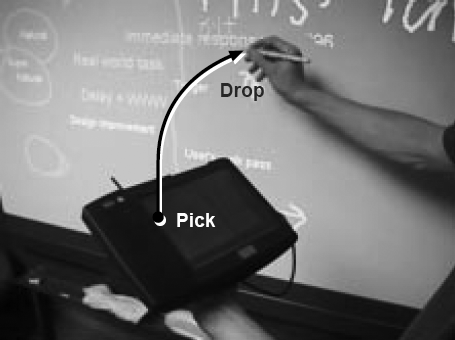
\includegraphics[width=6cm]{gfx/wboard.png}
	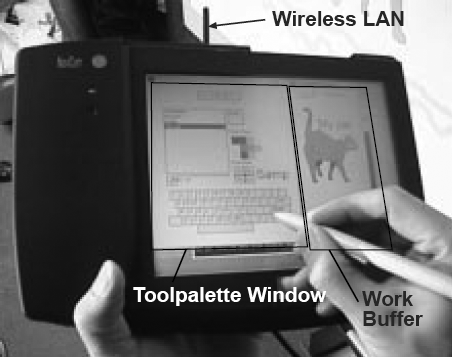
\includegraphics[width=6cm]{gfx/wboard2.png}
	\caption{Digital Whiteboard:
		Pick-and-drop interaction;
		Working areas for each participant's palmtop.}
	\label{FIG-WBOARD}
\end{figure}

The solution involves each participant carrying a pen and a palmtop,
with the pen working on both palmtop and whiteboard.
A direct manipulation method called Pick-and-drop(see Fig. \ref{FIG-WBOARD} left) was developed.
It allows a user to pick an object in his palmtop and dropping it on the whiteboard.
From the implementation point of view data is transferred through the network,
but from the user's perspective this technique allows him to pick up digital data
as if it were a physical object.
Text entry is performed on the palmtop and each user can choose the method he favors
(i.e.: handwritten recognition, soft keyboard, etc) for entering text.
No menus or tool palettes exist on the whiteboard -- they're available on each user's palmtop.
The main window is a multi page tool panel.
A user can flip to several tool palette pages, with the remaining area available as a temporary work buffer.
Users can store data elements in this window and paste them to the whiteboard
using Pick-and-Drop operations. (see Fig. \ref{FIG-WBOARD} right).

Rekimoto concludes that by putting many functions on palmtops,
users tend to concentrate too much on their own palmtop devices,
degrading mutual awareness among the participants.
Pick-and-Drop often worked better than drag-and-drop,
particularly when user had to move objects for a long distance.
Drag-and-drop forces a user to keep the pen tip in contact
with the board during the entire operation,
a restriction not suitable for large display surfaces.

%\paragraph{Discussion}

The solution where each user carries a palmtop for the creation of content such as note taking
is suitable for an architectural design and review scenario.
It grants the user the power to draw, type text or compose graphics 
independently from one another and then replicating the information on the whiteboard.
On the other hand there's the danger of users focusing too much on their paltop and losing
awareness of what's happening at the whiteboard.


\section{Approaches}

The set of available motion tracking techniques for gathering user input is discussed.
The most common setups for rendering virtual reality scenes are compared.
The shape creation projects Sesame and SmartPaper are analysed and three scene navigation concepts are visited.

\subsection{Input Modalities}

\subsubsection{Motion Tracking Systems}


Welch and Foxlin \cite{MT-BULLET} conducted a survey on motion tracking systems,
comparing each solution in terms of cost, precision and capacity to solve the tracking problem.
The main group of purposes for motion tracking applications was identified:
view control, navigation, object selection or manipulation, instrument tracking and avatar animation.
There are motion tracking systems available based on measurements of mechanical, inertial, acoustic, magnetic,
optical and radio frequency sensors, each approach bearing its advantages and limitations.
The most robust solution lies in combining two technologies,
such as a hybrid between inertial and acoustic sensors
-- the former providing 6 degrees of freedom data and the latter reading precise positioning for each artifact.

%\TODOL{BRIDGE WITH STT SYSTEM?, MORE INFO EXTRACTED FROM SOURCE?}

%\paragraph{Discussion}

One can envision the proposed solution to use motion tracking to allow users to change their
point of view in the program, navigate the scene, select and manipulate objects, a subset
of functionality identified by Welch and Foxlin.

\subsubsection{Augmented Reality versus Immersive Virtual Reality}

According to Azuma \cite{OVERVIEW-AR} Augmented Reality should be used
when the collaboration task is co-located,
when there is tangible object interaction and enhanced interaction in the real world.
Immersive Virtual Reality is preferred on scenarios with shared views and
remote collaboration.

%\TODOL{MORE CONTENT FROM THIS ARTICLE?}

%\paragraph{Discussion}
%There haven't been set any goals that force the Augmented Reality approach for such a system.
Sharing views and doing collaboration are two expected features of this system so
Virtual Reality is the choice to make. No Augmented Reality feature is found in this project.


%\TODO{issuing voice commands}
%\subsubsection{Voice Commands}
%
%\cite{SP-GEST-TTOP}

% OUTPUT MODALITIES
% using the tablet PC's display
% using a powerwall
% using HMDs

In order to obtain an immersive experience, there's a number of hardware
setups commonly available:

\begin{description}
	\item[Head-Mounted Display (HMD)] --
	  Head-mounting displays are glass-shaped devices, projecting a pair of stereo
	  transformed images to the user's retinas.
	  They normally feature a gyroscope or similar apparatus to measure head orientation and tilt.
	  There are two kinds of HMDs: in the former the images are projected in small opaque screens;
	  in the latter the projected surface is translucid, allowing blending of real and virtual worlds.
	  Translucid HMDs are best crafted for Augmented Reality (AR).
	  
		Using an HMD has the benefit of sticking to the user's head and detecting head orientation.
		On the other hand each HMD serves one single user and it has limited resolution.
		Additionally, most users report suffering from fatigue after long periods of
		usage \cite{VREDUC}.
		Opaque HMDs have the additional downside of users being unable to see the real world, 
		which can be confusing as noted by \cite{VANDERPOL}.
			
	\item[Cave Automatic Virtual Environment (CAVE)] --
	  A CAVE is an immersive virtual reality environment where projectors are directed to four,
	  five or all the six walls of a room-sized cube.
	  
		It shares the benefit of enclosing the user's viewing area with HMDs.
		Has a better resolution though.
		The downside is the small number of simultaneous users who can experience the CAVE at the same time.
	
	\item[Power Wall] --
	  A power wall is a large surface, usually planar, filled by an image.
	  The whole image projection is responsibility of a cluster of projectors set up in a wall.
	  Each projector renders part of the surface and the border between projections is ideally minimal.
	  Each projector is controlled by an independent computer.
	  
		Its size and resolution depend entirely on the setup, but normally a wall offers high resolution
		(depends on the number of projectors in the grid and each projector's resolution).
		Due to the large surface of the wall, several users may be served as once. Another benefit
		is users freedom of movement due to users not carrying wires \cite{INTTABLE}.
		The downside is users having to face the wall to experience the image entirely.
\end{description}

\begin{figure}[!ht]
	\centering
	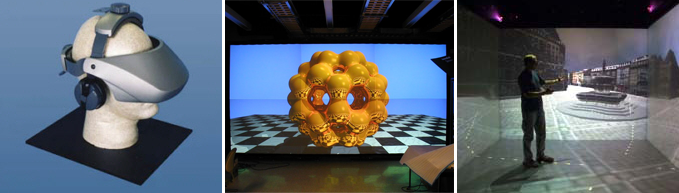
\includegraphics[width=12cm]{gfx/hmd-cluster-cave.png}
	\caption{HMD, Wall, CAVE}
	\label{FIG-HMD-CLUSTER-CAVE}
\end{figure}

Any of these setups is suitable for single user interaction.
In case of a reviewing session, in which at least two participants are required,
CAVE or Wall are better suited, since they alone offer a solution for a small group.

Using a Wall or CAVE presents other challenges: the computers responsible for
generating each projectors' images must be synchronized, its color parameters calibrated
and the viewport must be well cropped.
Several systems exist capable of delivering high performance 3D graphics and
offering the features mentioned above.
Based on scene graphs there are two well established solutions:
OpenSceneGraph\cite{SITE-OSG} and OpenSG\cite{SITE-OPENSG}.


\subsection{Shape Creation}

% SHAPE CREATION AND TRANSFORMATIONS
% for modeling simple buildings
% their translation, scaling, etc.
%\TODO{shape creation}
%\TODO{transformations}

In this section two solutions suitable for conceptual sketching of 3D forms are analyzed.

\subsubsection{SESAME, 2006}

Oh, Stuerzlinger and Danahy \cite{SESAME3D} developed SESAME
(Sketch, Extrude, Sculpt, and Manipulate Easily).
This system tries to provide an interface as powerful and easy to use as 2D sketching on paper.
It is defended by the authors that a 3D model is more easily understood between users
than a regular conceptual design.
It is optimized for modification and allows the creation and editing of volumetric geometry
by extruding 2D contours or sculpting 3D volumes.
It features an enhanced suggestive interface, allowing the creation of lines,
arcs and free-form curves with constraints.
SESAME also supports automatic grouping of objects, i.e., objects related
between themselves (ex: cup on top of table) affect each other.

The user tests conducted comparing SESAME against the popular modeling package
Autodesk 3D Studio Max show that even for experienced 3DSM users
the drawings done with SESAME were more creative and satisfying.

\begin{figure}[!ht]
	\centering
	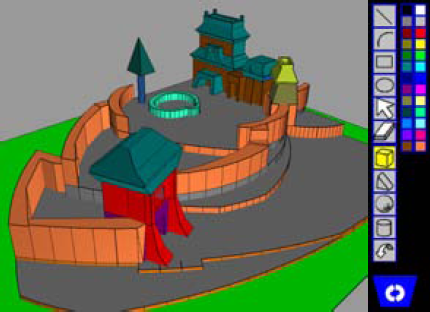
\includegraphics[width=6cm]{gfx/sesame.png}
	\caption{A view of a drawing done in 40 minutes with SESAME}
	\label{FIG-SESAME}
\end{figure}

\paragraph{Discussion}

This is a promising direction for an urban sketching software to go.
The tests against 3D Studio Max were a bit skewed -- the test should
have been conducted against a system of similar approach, such as Google Sketchup.
The offered interface in SESAME appears poorly thought out.

Some constraints may arise from applying these concepts to a multimodal collaborative
system.



\subsubsection{SmartPaper, 2004}

Shesh and Chen \cite{SMARTPAPER} developed SmartPaper, a system designed to support
2D sketching, featuring oversketching capabilities, sketch on 3D, 3D transforms and
CSG operations. It employs a non-photorealistic rendering technique to convey the
drawing a sketchy look.

\begin{figure}[!ht]
	\centering
	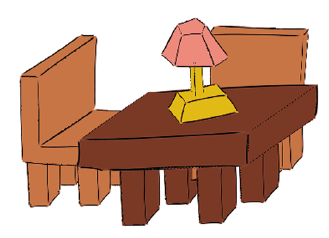
\includegraphics[width=5cm]{gfx/smartpaper.png}
	\caption{Drawing done with SmartPaper}
	\label{FIG-SMARTPAPER}
\end{figure}

\begin{figure}[!ht]
	\centering
	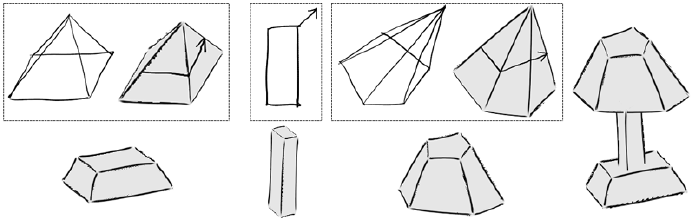
\includegraphics[width=8cm]{gfx/smartpaper2.png}
	\caption{The process of modeling a lamp in SmartPaper}
	\label{FIG-SMARTPAPER2}
\end{figure}

\paragraph{Discussion}

The biggest limitation found in SmartPaper is the lack of curved line support.
Another requirement is that the user must draw all object's edges, not only
the visible ones. In the case of extruded objects this is not problematic, since
the original face would always have to be drawn anyway.
The resulting geometry appears to be irregular but since the goal is to do
conceptual drawings this is not an issue.

\TODOL{RELATE TO OUR PROJECT?}


\subsection{Scene Navigation}


% SCENE NATIGATION

Following is a list of scene navigation solutions.
Each one can contribute to a more powerful and easy interface.


\subsubsection{Smart and Physically Based Camera, 2006}
\label{SMARTCAM-LABEL}

In order to ensure users not ``getting lost'' in the virtual space,
Buchholz, Bohnet and D�llner \cite{SMARTCAM} propose a smart and physically based camera.
Smart in the sense that it is aware of confusing and disorienting viewing situations,
providing means to circumvent them.
Physically based because it is supported by a physics model of 3D motion
to ensure steady, continuous user movements.

Experience shows that people frequently lose track of their location when moving on a 3 dimensional
world.
To solve this problem, the camera must identify situations when to intervene.
For that reason a metric, called orientation value, was created.
Each view is classified by counting its pixels, granting different values:
landmarks get the highest values; terrain gets mid-range values and the sky gets lower values (see Fig. \ref{FIG-SMARTCAM1}, right).
A threshold can then be established and views below the threshold are classified ``disoriented''.
When such an event takes place, smart navigation techniques restrict camera control.
The constraints posed to user control must be as comprehensible as possible.
Camera movement should also be time-coherent and physically sound.

The maintenance strategy solves critical situations such as (see Fig.\ref{FIG-SMARTCAM1}, left):

\begin{enumerate}[a)]
	\item The user rotates the flight direction and causes the camera to look too far beyond the terrain border.
		The rotation is accepted but outweighed by a slight rear movement away from the border.
	\item The user is flying forward beyond the terrain border.
		The maintenance strategy temporarily tilts down the view direction until a maximum angle is reached.
	\item If no more tilting is possible, the strategy rotates the flight direction parallel to the terrain
		to fly along the terrain border.
\end{enumerate}

\begin{figure}[!ht]
	\centering
	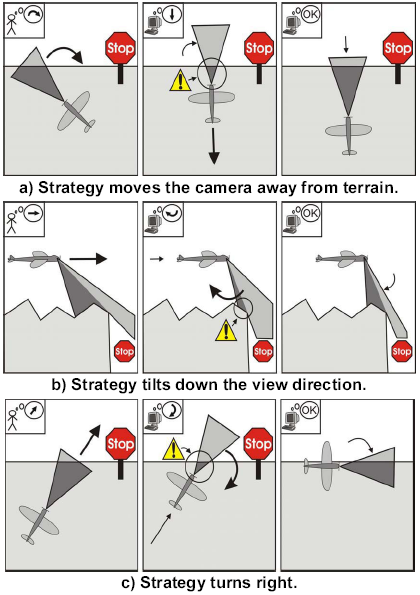
\includegraphics[height=7cm]{gfx/smartcam05-1.png}
	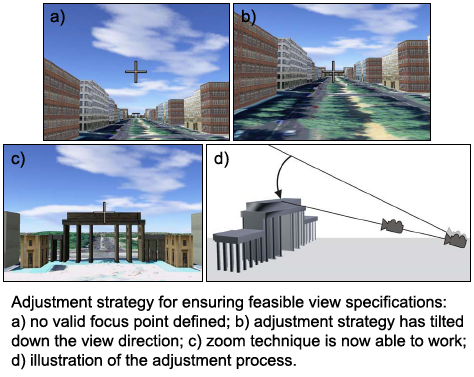
\includegraphics[height=5cm]{gfx/smartcam05-2.png}
	\caption{SPB Cam: Maintenance strategy for keeping high orientation values; Adjustment strategy for ensuring of feasible view specifications.}
	\label{FIG-SMARTCAM1}
\end{figure}

%\paragraph{Discussion}

A camera system such as this can be useful aiding non-experienced users such as clients in navigation tasks
since it maximizes the presence of landmarks in the user's view.
The physically-based engine would grant additional realism to the navigation experience, providing collision
detection, inertia and a spring behavior that would soften camera trajectories.



\subsubsection{Speed-dependent Automatic Zooming, 2000}
\label{SPEEDZOOM-LABEL}

Igarashi and Hinckley \cite{SPEEDZOOM} propose a simple idea for scrolling through large areas of information.
The speed at which the scrolling occurs changes the zooming of the seen area.
This makes sense since the faster the area is scrolling, the longer ahead the user needs to see.

%\paragraph{Discussion}

This could be easily applied to bird's-eye-view maps of large areas.
The scrolling of the map would trigger different zooming factors depending on
the scrolling speed, improving the navigation and exploration of the map.


\subsubsection{Path Drawing for 3D Walkthrough, 1998}
\label{PATH3D-LABEL}

Igarashi et al. \cite{PATH3D} start by identifying the two main types of walkthrough techniques:
\emph{driving}, where the user continuously changes camera position with move and rotation buttons and
\emph{flying}, where the user picks the desired destination with a pointing device and a trajectory is calculated
and animated from the starting position to the picked one.
Each has it disadvantages:
driving requires the user to control the trajectory at all times;
flying lacks expressive power since the user can't control the path neither the final orientation.

The proposed solution is an extension of the flying technique:
the user draws the desired path he wants to take on the screen.
It gets projected onto the walking surfaces and the generated path is animated.
During the animation the user faces the tangential direction related to the path.
This brings the additional advantage of the user being able to define
where he will be facing at the end of the animation.
This technique can be used is two different ways.
The user can draw a long stroke specifying the path at once
or he can draw successions of small strokes (see Fig.\ref{FIG-PATH3D}).

As limitations the authors state the path expressiveness
being limited to the walking surface planes
and the need for the user's avatar to be present on the view
if one wants to draw the path from the user's feet.
 

\begin{figure}[!ht]
	\centering
	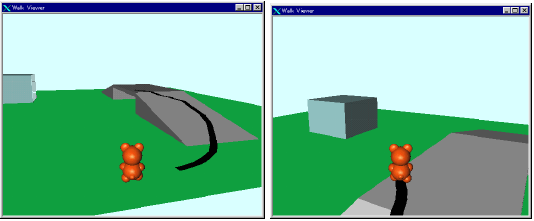
\includegraphics[width=12cm]{gfx/path3d.png}
	\caption{One long path and one short one}
	\label{FIG-PATH3D}
\end{figure}

%\paragraph{Discussion}

This navigation mode could be handy in the review scenario.
Even so this might be hard to apply to the project due to LSD interface limitations.


